\chapter{Modal logic}

\section{Syntax and semantics}

Here we reintroduce the syntax and semantics of the logic \logicKF{}, as
introduced by van Ditmarsch and French~\cite{french2009simulation}.

% TODO - more motiviation

\begin{definition}[Language of \langF{}] % TODO - move to the K section
Given a finite set of agents $A$ and a set of propositional atoms $P$, the
language of \langF{} is defined by the following abstract syntax:

$$
\phi ::=    p \bnfalt
            \neg \phi \bnfalt
            \phi \land \phi \bnfalt
            \knows_a \phi \bnfalt
            \allrefs_a \phi
$$
where $a \in A$ and $p \in P$.
\end{definition}

Standard abbreviations include:
$\top ::= \phi \lor \neg \phi$;
$\bot ::= \neg \top$;
$\phi \lor \psi ::= \neg (\neg \phi \land \neg \psi)$;
$\phi \implies \psi ::= \neg \phi \lor \psi$;
and $\suspects_a \phi ::= \neg \knows_a \neg \phi$.
We use an abbreviation for the dual of the $\allrefs_a$ operator,
$\somerefs_a \phi ::= \neg \allrefs_a \neg \phi$.

We also use the cover operator $\covers_a \Gamma$, where $\Gamma$ is a finite
set of formulae, which is an abbreviation for 
$\covers_a \Gamma ::= \knows_a \bigvee_{\gamma \in \Gamma} \gamma \land
\bigwedge_{\gamma \in \Gamma} \suspects_a \gamma$. The cover operator is relied
on for our axiomatisation, in much the same way it is relied on for the
axiomatisation of \logicKiF{} presented by van Ditmarsch, French and
Pinchinat~\cite{french2010future}. % TODO - include citation for cover operator

\begin{definition}[Semantics of \logicKF{}]
Let $M = (S, R, V)$ be a Kripke model. The interpretation of $\phi \in
\logicKF$ is defined inductively.

\begin{eqnarray*}
M_s &\entails& p \text{ iff } s \in V_p\\
M_s &\entails& \neg \phi \text{ iff } M_s \nentails \phi\\
M_s &\entails& \phi \land \psi \text{ iff } M_s \entails \phi \text{ and } M_s
\entails \psi\\
M_s &\entails& \knows_a \phi \text{ if for all } t \in S : (s, t) \in R_a \text{
implies } M_t \entails \phi\\
M_s &\entails& \allrefs_a \phi \text{ iff for all } M'_{s'} \in \classK : M_s
\simulation_a M'_{s'} \text{ implies } M'_{s'} \entails \phi\\
\end{eqnarray*}
\end{definition}

% TODO - remark about logic

\begin{lemma}
The logic \logicKF{} is bisimulation invariant.
\end{lemma}

This is proven by van Ditmarsch, French and Pinchinat~\cite{french2010future}.

% TODO - examples

In previous work, van Ditmarsch, French and Pinchinat gave an axiomatisation of
the single-agent variant of \logicKF{}, called \logicKiF{}. The axiomatisation
was formulated in terms of the cover operator, $\covers$, an abbreviation
introduced previously. The completeness proof consisted of a translation of
\logicKiF{} formulae into \logicKi{} formulae, a translation which relied on the
formulae being in a disjunctive normal form, using the cover operator. Our
axiomatisation for the multi-agent logic \logicKF{} relies on the same
disjunctive normal form, which we will define now.

\begin{definition}[Disjunctive normal form]
A formula in disjunctive normal form is defined by the following abstract syntax:

$$
\alpha ::= \pi \land \bigwedge_{a \in A} \covers_a \Gamma_a \bnfalt \alpha \lor \alpha
$$
where $\pi$ stands for a propositional formula, $a \in A$, and $\Gamma_a$ stands
for a finite set of formulae in disjunctive normal form.
\end{definition}

\begin{lemma}\label{k-dnf}
Every well-formed formula of \logicK{} is equivalent to a formula in disjunctive
normal form.
\end{lemma}

\begin{proof}
Let $\phi$ be a \logicK{} formula. We use an inductive argument over the
structure of $\phi$ to show that it can be converted into cover disjunctive
normal form.

The base case is where $\phi$ is a propositional formula. Then we can add
vacuous cover operators of the form $\covers_a \{\top\}$ for each $a \in A$ to
yield a formula in disjunctive normal form.

Suppose that $\phi$ contains conjuncts of the form $\knows_a \gamma$ or
$\suspects_a \gamma$. By the induction hypothesis we may assume that $\gamma$ is
in disjunctive normal form. Then we can convert these terms using the
equivalences $\knows_a \gamma \equiv \covers_a \{\gamma\} \lor \covers_a
\emptyset$ and $\suspects_a \gamma \equiv \covers_a \{\gamma, \top\}$. We can
add vacuous cover operators of the form $\covers_a \{\top\}$ for any agent $a
\in A$ which is not represented in each disjunct of $\phi$.

An inductive argument can be used to show that we can collapse the resulting
conjunction of cover operators so that each agent is represented by a cover
operator only once. We use the following equivalence to achieve this.

$$
\covers_a \Gamma \land \covers_a \Gamma' \equiv 
\covers_a \big( 
\{ \gamma \land \bigvee_{\gamma' \in \Gamma'} \gamma' \mid \gamma \in \Gamma \}
\cup
\{ \gamma' \land \bigvee_{\gamma \in \Gamma} \gamma \mid \gamma' \in \Gamma' \}
\big)
$$

We note that as each $\gamma \in \Gamma$ and $\gamma' \in \Gamma'$ are assumed
to be disjunctive normal formulae, that applying a disjunction over each of
these sets yields a disjunctive normal formula. Conjoining two disjunctive
normal formulae does not yield a disjunctive normal formula, however we note
that we can use the distributivity of conjunction over disjunction, and then
recursively collapse the duplicated cover operators, to yield a formula in
disjunctive normal form.

Repeating this for each disjunct in our original formula leaves us with a
formula in cover logic disjunctive normal form.
\end{proof}

\section{Axiomatisation}

\begin{definition}[\axiomKF]
The axiomatisation \axiomKF{} is a substitution schema consisting of the
following axioms:

$$
\begin{array}{rl}
{\bf P} & \text{All propositional tautologies}\\
{\bf K} & \knows (\phi \implies \psi) \implies \knows \phi \implies \knows
\psi\\
{\bf R} & \allrefs_a (\phi \implies \psi) \implies \allrefs_a \phi \implies
\allrefs_a \psi\\
{\bf RP} & \allrefs_a \alpha \iff \alpha \text{ where $\alpha$ is a
propositional formula}\\
{\bf RComm} & \somerefs_a \covers_b \Gamma \iff \covers_b \{\somerefs_a \gamma
\mid \gamma \in \Gamma\} \text{ where $a \neq b$}\\
{\bf RDist} & \bigwedge_{b \in A} \somerefs_a \covers_b \Gamma_b \implies
\somerefs_a \bigwedge_{b \in A} \covers_b \Gamma_b\\
{\bf RK} & \somerefs_a \covers_a \Gamma \iff \bigwedge_{\gamma \in \Gamma}
\suspects_a \somerefs_a \gamma\\
\end{array}
$$

Along with the rules:

$$
\begin{array}{rl}
{\bf MP} & \text{From $\proves \phi \implies \psi$ and $\proves \phi$, infer
$\proves \psi$}\\
{\bf NecK} & \text{From $\proves \phi$ infer $\proves \knows_a \phi$}\\
{\bf NecR} & \text{From $\proves \phi$ infer $\proves \allrefs_a \phi$}
\end{array}
$$
\end{definition}

\begin{lemma}\label{k-sound}
The axiomatisation \axiomKF{} is sound in \logicKF{}.
\end{lemma}

\begin{proof}
The soundness of the axioms {\bf P}, and {\bf K}, and the rules {\bf MP} and
{\bf NecK} can be shown by the same reasoning used to show that they are sound
in \logicK{}. The soundness of the axioms {\bf RP} and {\bf R}, and the rule
{\bf NecR} can be shown by the same reasoning used to how that they are sound in
the logic \logicKiF{}~\cite{french2010future}.

All that remains to be shown is the soundness of {\bf RK}, {\bf RComm}, and {\bf
RDist}.

\paragraph{RK}
Suppose that $M_s$ is a Kripke model such that $M_s \entails \bigwedge_{\gamma
\in \Gamma} \suspects_a \somerefs_a \gamma$, where $\Gamma$ is a non-empty set
of formulae.

Then consider $\gamma \in \Gamma$. From $M_s \entails \suspects_a \somerefs_a
\gamma$, there exists a state $s^\gamma \in sR^M$ such that $M_{s^\gamma}
\entails \somerefs_a \gamma$. Therefore there exists a Kripke model
$N^\gamma_{t^\gamma} \refinement_a M_{s^\gamma}$, via some $a$-simulation
$\mathcal{R}^\gamma$, such that $N^\gamma_{t^\gamma} \entails \gamma$.

Without loss of generality we assume that each $N^\gamma$ is disjoint.

Let $t \notin S^M$ and $t \notin S^{N^\gamma}$ for every $\gamma \in \Gamma$.
Then we construct a Kripke model $N = (S^N, R^N, V^N)$ where:

\begin{eqnarray*}
S^N &=& \{t\} \cup S^M \cup \bigcup_{\gamma \in \Gamma} S^{N^\gamma}\\
R^N_a &=& \{(t, t^\gamma) \mid \gamma \in \Gamma\}
\cup R^M_a
\cup \bigcup_{\gamma \in \Gamma} R^{N^\gamma}_a\\
R^N_b &=& \{(t, t') \mid t' \in sR^M_b\}
\cup R^M_b
\cup \bigcup_{\gamma \in \Gamma} R^{N^\gamma}_b \text{ for $b \in A - \{a\}$}\\
V^N(p) &=& 
\begin{cases}
\{t\} \cup V^M(p) \cup \bigcup_{\gamma \in \Gamma} V^{N^\gamma}(p) & \text{if $s
\in V^M(p)$}\\
V^M(p) \cup \bigcup_{\gamma \in \Gamma} V^{N^\gamma}(p) & \text{otherwise}
\end{cases}
\text{ for $p \in P$}
\end{eqnarray*}

\begin{figure}
\begin{center} % TODO - better diagram
\scalebox{0.4}{
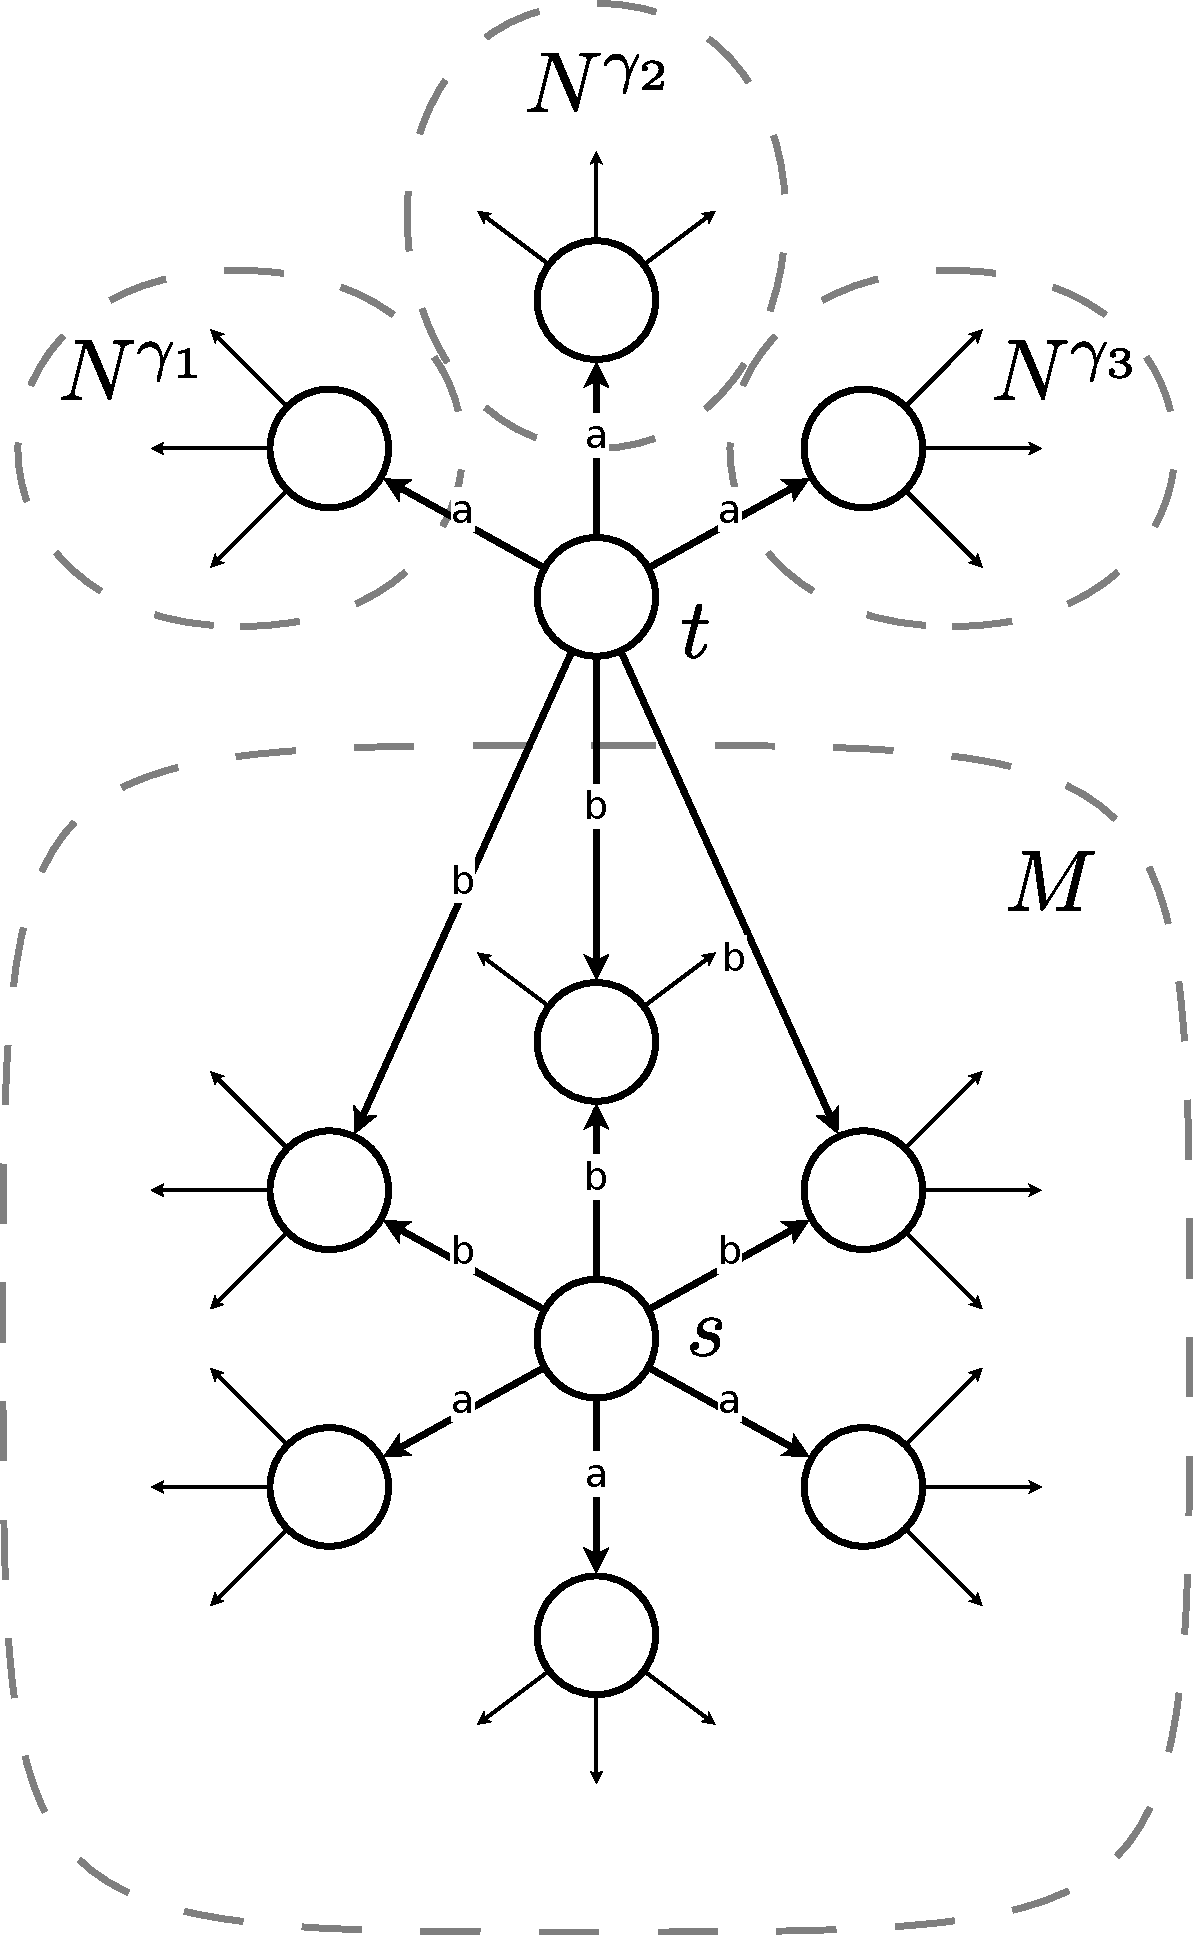
\includegraphics{rk}
}
\caption{
The model $N$ is constructed by taking the model $M$ and the models $N^\gamma$
for every $\gamma \in \Gamma$, and connecting them with an extra node $t$. $t$
is connected via an $a$-edge to $t^\gamma$ from each of the $N^\gamma$, and is
also connected via a $b$-edge to each $b$-successor of $s$ in $M$.
}
\end{center}
\end{figure}

We must show that $N_t$ is an $a$-refinement of $M_s$, and that for every
$t^\gamma \in tR^N_a$ we have that $N_{t^\gamma} \entails \gamma$. The latter
will be shown by proving that for every $\gamma \in \Gamma$, the state
$N_{t^\gamma}$ is bisimilar to $N^\gamma_{t^\gamma}$.

First we must show that $N_t$ is an $a$-refinement of $M_s$. We construct an
$a$-simulation $\mathcal{R}$ from $N_t$ to $M_s$, where:

$$\mathcal{R} = \{(t, s)\} \cup \{(s', s') \mid s' \in S^M \} 
\cup \bigcup_{\gamma \in \Gamma} \mathcal{R}^\gamma$$

We must show that $\mathcal{R}$ satisfies {\bf atoms}, {\bf forth-$b$} for every
$b \in A$, and {\bf back-$b$} for every $b \in A - \{a\}$.

We note that, by construction, the valuation of $N$ matches the valuation of its
corresponding states in $M$ and each $N^\gamma$, and the valuation of $N_t$
matches that of $M_s$. Therefore $\mathcal{R}$ satisfies {\bf atoms}.

We next show that $\mathcal{R}$ satisfies {\bf forth-$b$} for every $b \in A$.
Let $b \in A$, $u \in S^N$ and $v \in S^M$ such that $(u, v) \in \mathcal{R}$.
Suppose that $(u, v) \in \mathcal{R}^\gamma$ for some $\gamma \in \Gamma$.
Then as $\mathcal{R}^\gamma$ is an $a$-simulation, it satisfies {\bf forth-$b$}
for every $b \in A$. Hence for every $u' \in uR^{N^\gamma}_b$, there exists some
$v' \in vR^M_b$ such that $(u', v') \in \mathcal{R}^\gamma \subseteq
\mathcal{R}$. Suppose that $b = a$ and $u = t^\gamma$ for some $\gamma \in
\Gamma$.  Suppose instead that $(u, v) = (s', s')$ for some $s' \in S^M$.  Then
we note that $s'R^N_b = s'R^M_b$, and hence for every $s'' \in s'R^N_b$ we have
that $s'' \in s'R^M_b$, and that $(s'', s'') \in \mathcal{R}$. Finally suppose
that $(u, u') = (t, s)$. Then suppose that $b = a$. By construction, $tR^N_a =
\{t^\gamma \mid \gamma \in \Gamma\}$, and hence $v = t^\gamma$ for some $\gamma
\in \Gamma$. Hence we can take $s^\gamma \in sR^M_a$, and note that as
$\mathcal{R}^\gamma$ is an $a$-simulation from $M_{s^\gamma}$ to
$N^\gamma_{t^\gamma}$, we know that $(t^\gamma, s^\gamma) \in \mathcal{R}^\gamma
\subseteq \mathcal{R}$. Suppose that $b \neq a$. Then by construction, $tR^M_b =
sR^M_b$, hence for every $t' \in tR^M_b$, we have that $t' \in sR^M_b$, and
hence we know that $(t', t') \in \mathcal{R}$. Hence $\mathcal{R}$ satisfies
{\bf back-$b$} for every $b \in A$.

A similar argument to above shows that $\mathcal{R}$ satisfies {\bf forth-$b$}
for every $b \in A - \{a\}$.

We next show that for every $\gamma \in \Gamma$, we have that $N_{t^\gamma}
\entails \gamma$. We show this by showing that $N_{t^\gamma}$ is bisimilar to
$N^\gamma_{t^\gamma}$. This is clear as $N$ contains a duplicate of the states
and edges of each $N^\gamma$, and the only additional edges in $N$ that are not in
$N^\gamma$ are from $t$ to $t^\gamma$. Therefore, as for every $\gamma \in
\Gamma$, we have that $N^\gamma_{t^\gamma} \entails \gamma$, by bisimulation
invariance we also have that $N_{t^\gamma} \entails \gamma$. Hence $N_t \entails
\covers_a \Gamma$.

As $N_t \refinement_a M_s$, and $N_t \entails \covers_a \Gamma$ we therefore
have that $M_s \entails \somerefs_a \covers_a \Gamma$.

Conversely, suppose that $M_s \entails \covers_a \Gamma$. Then there exists a
Kripke model $N_t \refinement_a M_s$, via some $a$-simulation $\mathcal{R}$,
such that $N_t \entails \covers_a \Gamma$. From the definition of the cover
operator, this implies that $N_t \entails \knows_a \bigvee_{\gamma \in \Gamma}
\gamma \land \bigwedge_{\gamma \in \Gamma} \suspects_a \gamma$. In particular we
note that for every $\gamma \in \Gamma$, $N_t \entails \suspects_a \gamma$, and
so there exists some $t^\gamma \in tR^N_a$ such that $N_{t^\gamma} \entails
\gamma$. As $t^\gamma \in tR^N_a$, and $(t, s) \in \mathcal{R}$, by {\bf
forth-$a$} there exists some $s^\gamma \in sR^M_a$ such that $(t^\gamma, s^\gamma)
\in \mathcal{R}$. Hence $\mathcal{R}$ is also an $a$-simulation from
$N_{t^\gamma}$ to $M_{s^\gamma}$, and so $M_{s^\gamma} \entails \somerefs_a
\gamma$. As for every $\gamma \in \Gamma$ we have that $s^\gamma \in sR^M_a$, we
also have that $M_s \entails \suspects_a \somerefs_a \gamma$. Therefore we
finally have that $M_s \entails \bigwedge_{\gamma \in \Gamma} \suspects_a
\somerefs_a \gamma$.

Therefore {\bf RK} is sound.

\paragraph{RComm}
Suppose that $M_s$ is a Kripke model such that $M_s \entails \covers_b \{
\somerefs_a \gamma \mid \gamma \in \Gamma\}$, where $a \ne b$, and $\Gamma$ is a
finite set of formulae. From the definition of the cover operator, this implies
that $M_s \entails \knows_b \bigvee_{\gamma \in \Gamma} \somerefs_a \gamma \land
\bigwedge_{\gamma \in \Gamma} \suspects_b \somerefs_a \gamma$. In particular, we
note that for every $\gamma \in \Gamma$, there exists some $s^\gamma \in sR^M_b$
such that $M_{s^\gamma} \entails \somerefs_a \gamma$.  Then there exists a
Kripke model $N^\gamma_{t^\gamma} \refinement_a M_{s^\gamma}$, via some
$a$-simulation $\mathcal{R}^\gamma$, such that $N^\gamma_{t^\gamma} \entails
\gamma$. Without loss of generality we may assume that the $N^\gamma$ are
disjoint.

Let $t$ be a state such that $t \notin S^{N^\gamma}$ for every $\gamma \in
\Gamma$. Then we construct a Kripke model $N = (S^N, R^N, V^N)$, where:

\begin{eqnarray*}
S^N &=& \{t\} \cup S^M \bigcup_{\gamma \in \Gamma} S^{N^\gamma}\\
R^N_b &=& \{(t, t^\gamma) \mid \gamma \in \Gamma\} 
\cup  R^M_b 
\cup \bigcup_{\gamma \in \Gamma} R^{N^\gamma}_b\\
R^N_c &=& \{(t, t') \mid t' \in sR^M_c\} 
\cup R^M_c \cup \bigcup_{\gamma \in \Gamma} R^{N^\gamma}_c \text{ for $c \in A - \{b\}$}\\
V^N(p) &=& 
\begin{cases}
\{t\} \cup V^M(p) \cup \bigcup_{\gamma \in \Gamma} V^{N^\gamma}(p) & \text{if $s
\in V^M(p)$}\\
V^M(p) \cup \bigcup_{\gamma \in \Gamma} V^{N^\gamma}(p) & \text{otherwise}
\end{cases}
\text{ for $p \in P$}
\end{eqnarray*}

We construct an $a$-simulation $\mathcal{R}$ from $N_t$ to $M_s$, where:

$$\mathcal{R} = \{(t, s)\} \cup \{(s', s') \mid s' \in S^M\} \cup
\bigcup_{\gamma \in \Gamma} \mathcal{R}^\gamma$$

We note that $\mathcal{R}$ is an $a$-simulation, by similar arguments as used in
the proof for {\bf RK}. In particular, this means that $N_t \refinement_a M_s$.

We also note that for every $\gamma \in \Gamma$ that $N_{t^\gamma} \bisim
N^\gamma_{t^\gamma}$, by similar arguments as used in the proof for {\bf RK}.
In particular, this means that as $N^\gamma_{t^\gamma} \entails \gamma$ that we
also have $N_{t^\gamma} \entails \gamma$, for every $\gamma \in \Gamma$.
Therefore $N_t \entails \covers_b \Gamma$.

Therefore $M_s \entails \somerefs_a \covers_b \Gamma$.

The converse, $\somerefs_a \covers_b \Gamma \implies \covers_b \{\somerefs_a
\gamma \mid \gamma \in \Gamma\}$ follows a similar proof to the relevant part in
the proof for {\bf RK}.

Therefore {\bf RComm} is sound.

\paragraph{RDist}
Suppose that $M_s$ is a Kripke model such that $M_s \entails \bigwedge_{b \in A}
\somerefs_a \covers_b \Gamma_b$, where $\Gamma_b$ is a finite set of formulae
for each $b \in A$.

Then as $a \in A$, we have that $M_s \entails \somerefs_a \covers_a \Gamma_a$,
and by {\bf RK} this implies that $M_s \entails \bigwedge_{\gamma \in
\Gamma_a} \suspects_a \somerefs_a \gamma$. We also have for every $b \in A -
\{a\}$ that $M_s \entails \somerefs_a \covers_b \Gamma_b$, and by {\bf RComm}
this implies that $M_s \entails \covers_b \{\somerefs_a \gamma \mid \gamma \in
\Gamma_b\}$, and by the definition of the cover operator implies that $M_s
\entails \bigwedge_{\gamma \in \Gamma_b} \suspects_b \somerefs_a \gamma$.  Hence
for every $b \in A$ and $\gamma \in \Gamma_b$, we have that $\suspects_b
\somerefs_a \gamma$. This implies that for each $b \in A$ and each $\gamma \in
\Gamma_b$ that there exists some $t^{\gamma} \in sR^M_b$ such that $M_{t^\gamma}
\entails \somerefs_a \gamma$. Therefore there exists a Kripke model
$N^\gamma_{t^\gamma} \refinement_a M_{t^\gamma}$, via some $a$-simulation
relation $\mathcal{R}^\gamma$, such that $N^\gamma_{t^\gamma} \entails \gamma$.
Without loss of generality we may assume that the $N^\gamma$ are disjoint.

Let $t \notin S^{N^\gamma}$ for every $\gamma \in \Gamma$.
Then we construct a Kripke model $N = (S, R^N, V^N)$ where:

\begin{eqnarray*}
S^N &=& \{t\} \cup \bigcup_{b \in A, \gamma \in \Gamma_b} S^{N^\gamma}\\
R^N_b &=& \{(t, t^{\gamma}) \mid b \in A, \gamma \in \Gamma_b\} 
\cup \bigcup_{b \in A, \gamma \in \Gamma_b} R^{N^\gamma}_b \text{ for $b \in A$}\\
V^N(p) &=& 
\begin{cases}
\{t\} \cup \bigcup_{b \in A, \gamma \in \Gamma_b} V^{N^\gamma}(p) & \text{if $s
\in V^M(p)$}\\
\bigcup_{b \in A, \gamma \in \Gamma_b} V^{N^\gamma}(p) & \text{otherwise}
\end{cases}
\end{eqnarray*}

We construct an $a$-simulation $\mathcal{R}$ from $N_t$ to $M_s$, where:

$$\mathcal{R} = \{(t, s)\} \cup \bigcup_{b \in A, \gamma \in \Gamma_b}
\mathcal{R}^\gamma$$

We note that this is an $a$-simulation, by similar arguments as used in the
proof for {\bf RK}. In particular, this means that $N_t \refinement_a M_s$.

We also note that for every $b \in A$, and $\gamma \in \Gamma_b$ that
$N_{t^\gamma} \bisim N^\gamma_{t^\gamma}$, by similar arguments as used in the
proof for {\bf RK}. In particular, this means that as $N^\gamma_{t^\gamma}
\entails \gamma$ that we also have $N_{t^\gamma} \entails \gamma$, for every $b
\in A$ and $\gamma \in \Gamma_b$. Therefore $N_t \entails \covers_b \Gamma_b$
for every $b \in A$, and therefore $N_t \entails \bigwedge_{b \in A} \covers_b
\Gamma_b$.

Therefore $M_s \entails \somerefs_a \bigwedge_{b \in A} \covers_b \Gamma_b$ and
{\bf RDist} is sound.

Therefore the axiomatisation \axiomKF{} is sound.
\end{proof}

\begin{lemma}
The following is derivable in \axiomKF{}.

$$
\proves \bigwedge_{b \in A} \somerefs_a \covers_b \Gamma_b \iff
\somerefs_a \bigwedge_{b \in A} \covers_b \Gamma_b \\
$$
where $\Gamma_b$ is a set of $b$-disjunctive normal formulae for
every $b \in A$.
\end{lemma}

\begin{proof}
The forward direction is the axiom {\bf RDist}. 

The converse can be derived in a more general form as $\somerefs_a (\phi \land
\psi) \implies \somerefs_a \phi \land \somerefs_a \psi$. The derivation is
similar to the derivation for $\knows_a (\phi \land \psi) \implies \knows_a \phi
\land \knows_a \psi$ in the modal logic \logicK{}, using the axiom {\bf R} in
place of {\bf K}.
\end{proof}

\begin{lemma}\label{k-translation}
Every formula of \logicKF{} is provably equivalent to a formula of \logicK{}.
\end{lemma}

\begin{proof}
Given a formula $\psi$ we prove by induction on the number of occurrences of
\somerefs{} that $\psi$ is equivalent to a \somerefs-free formula, and
therefore to a formula in \logicK{}. The base case with no \somerefs operators
is trivial, as a \somerefs-free formula is a formula in \logicK{}. Now assume
that $\psi$ contains $n + 1$ \somerefs-operators. Choose a subformula of type
$\somerefs_a \phi$ of our given formula, where $\phi$ is \somerefs-free. Without
loss of generality, by Lemma~\ref{k-dnf} we may assume that $\phi$ is in
disjunctive normal form.  We prove by induction on the structure of $\phi$ that
$\somerefs_a \phi$ is provably equivalent to a formula $\chi$ without the
$\somerefs_a$ operator.

\begin{itemize}
\item $\somerefs_a (\phi \lor \psi)$ iff $\somerefs \phi \lor \somerefs \psi$.
(Derivable from {\bf P} and {\bf R})
\item $\somerefs_a (\pi \land \bigwedge_{b \in A} \covers_b \Gamma_b)$ iff
$\pi \land \bigwedge_{\gamma \in \Gamma_a} \suspects_a \somerefs_a \gamma \land
\bigwedge_{b \in A - \{a\}} \covers_b \{\somerefs_a \gamma \mid \gamma \in
\Gamma_b\}$ (Derivable from {\bf P}, {\bf R}, {\bf RP}, {\bf RDist}, {\bf
RK} and {\bf RComm})
\end{itemize}

Replacing $\somerefs_a \phi$ with $\chi$ in $\psi$ gives an equivalent formula
with one less \somerefs-operator. Thus by induction, all formulae in \logicKF{}
can be translated into an equivalent formula in \logicK{}.
\end{proof}

The rest of the completeness proof is merely a formality to show that, given the
above translation into \logicK{}, we can show completeness by using these
translations along with the completeness of \logicK{}.

\begin{corollary}\label{k-derivable}
Let $\phi \in \logicKF$ be given and $\psi \in \logicK$ be semantically
equivalent to $\phi$.  If $\psi$ is a theorem in \logicK{}, then $\phi$ is a
theorem in \axiomKF{}.
\end{corollary}

\begin{proof}
Let $\phi \in \logicKF$ and let $\psi \in \logicK$ be semantically equivalent to
$\phi$. By Lemma~\ref{k-translation}, we can obtain some $\phi' \in \logicK$
that is semantically equivalent to $\phi$ (and thus also to $\psi$) by following
the given translation steps. We can extend a derivation of $\psi$ to a
derivation of $\phi'$ as the two are semantically equivalent in \logicK{}, and by
the completeness of \logicK{} this equivalence is derivable. As \axiomKF{} is a
conservative extension of \logicK{}, this equivalence is therefore also derivable
in \axiomKF{}. The derivation can be further extended to $\phi$ by observing that all
of the reduction steps in Lemma~\ref{k-translation} are provable equivalences
in \axiomKF{}. Therefore $\phi$ is a theorem in \axiomKF{}.
\end{proof}

\begin{lemma}\label{k-complete}
The axiom schema \axiomKF{} is complete for the logic \logicKF{}.
\end{lemma}

Note that as we are discussing derivability in two different logics in the
following proof, we use a subscript on the turnstile symbol to denote the logic
we are working in (e.g. $\proves_{\logicKF}$)

\begin{proof}
Let $\phi \in \logicKF$ such that $\entails_{\logicKF} \phi$. Then by
Lemma~\ref{k-translation}, there exists a semantically equivalent formula
$\psi \in \logicK$ which is \somerefs-free. As $\entails_{\logicKF} \phi$ and
$\phi \iff \psi$, then $\entails_{\logicKF} \psi$. As $\psi$ is
\somerefs-free, then it follows that $\entails_{\logicK} \psi$, and by the
completeness of \axiomKF{} it follows that $\proves_{\logicK} \psi$.
Therefore by Corollary~\ref{k-derivable} we have that $\proves_{\logicKF}
\phi$.
\end{proof}

\begin{theorem}
The axiomatisation \axiomKF{} is sound and complete for the logic \logicKF{}.
\end{theorem}

\begin{proof}
The soundness proof is given in Lemma~\ref{k-sound} and the completeness
proof is given in Lemma~\ref{k-complete}.
\end{proof}
